\documentclass[tikz,border=10pt]{standalone}
\usetikzlibrary{arrows.meta,positioning}
\pagecolor{white}
\begin{document}
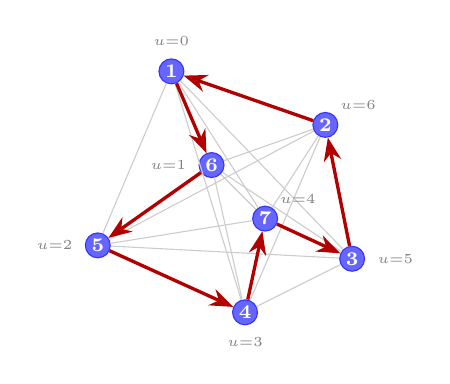
\begin{tikzpicture}[scale=0.85,
  city/.style={circle, draw=blue!80, fill=blue!60, inner sep=0pt,
               minimum size=9pt, font=\scriptsize\bfseries, text=white},
  tour/.style={very thick, red!70!black},
  nontour/.style={thin, gray!40}
]
  \node[city] (c1) at (-0.3, 2.3)  {1};
  \node[city] (c2) at (2.0, 1.5)   {2};
  \node[city] (c3) at (2.4,-0.5)   {3};
  \node[city] (c4) at (0.8,-1.3)   {4};
  \node[city] (c5) at (-1.4,-0.3)  {5};
  \node[city] (c6) at (0.3, 0.9)   {6};
  \node[city] (c7) at (1.1, 0.1)   {7};
  \foreach \i in {1,...,7} {
    \foreach \j in {\i,...,7} {
      \ifnum\i<\j
        \draw[nontour] (c\i) -- (c\j);
      \fi
    }
  }
  \draw[tour, -{Stealth}] (c1) -- (c6);
  \draw[tour, -{Stealth}] (c6) -- (c5);
  \draw[tour, -{Stealth}] (c5) -- (c4);
  \draw[tour, -{Stealth}] (c4) -- (c7);
  \draw[tour, -{Stealth}] (c7) -- (c3);
  \draw[tour, -{Stealth}] (c3) -- (c2);
  \draw[tour, -{Stealth}] (c2) -- (c1);
  \node[font=\tiny, gray, above=1pt of c1] {$u{=}0$};
  \node[font=\tiny, gray, left=1pt of c6] {$u{=}1$};
  \node[font=\tiny, gray, left=1pt of c5]  {$u{=}2$};
  \node[font=\tiny, gray, below=1pt of c4] {$u{=}3$};
  \node[font=\tiny, gray, above right=-2pt of c7] {$u{=}4$};
  \node[font=\tiny, gray, right=1pt of c3] {$u{=}5$};
  \node[font=\tiny, gray, above right=-2pt of c2] {$u{=}6$};
\end{tikzpicture}
\end{document}
